\documentclass[a4paper]{article}
\usepackage[utf8]{inputenc}
\usepackage[T1]{fontenc}
\usepackage[intlimits]{amsmath}
\usepackage{amsfonts}
\usepackage{amssymb}
\usepackage[export]{adjustbox}
\usepackage{graphicx}
\setlength{\parindent}{0pt}
\usepackage[left=1in, right=1in, top=1in, bottom=1in]{geometry}
\usepackage{float}
\usepackage{multicol}
\usepackage{listings}
\usepackage{xcolor}
\usepackage{cancel}
\usepackage{bm}
\usepackage{hyperref}
\setcounter{tocdepth}{1}
\usepackage[titletoc]{appendix}
\hypersetup{
	colorlinks=true,
	linkcolor=blue,
	filecolor=blue,
	urlcolor=blue,
}

\newcommand\blfootnote[1]{%
	\begingroup
	\renewcommand\thefootnote{}\footnote{#1}%
	\addtocounter{footnote}{-1}%
	\endgroup
}

\begin{document}
	
	\Huge\textbf{Beam Bend Calculator}
	\newline
	\LARGE AMB Calculator
	
	\vspace{0.5cm}
	\normalsize
	
	This calculator is used to check the deflection or twist in a beam (extrusion of uniform cross-section). It can be helpful for determining whether a profile or axle will be strong enough to carry the desired load. Note that this is not a replacement for proper Finite Element Analysis simulation and does not return the material stress.
	
	\section*{Material \& Cross-Section}
	
	Materials are defined with three values: Young's Modulus $ E $, Shear Modulus $ G $, and density $ \rho $. You can choose one of the pre-defined materials or enter these values manually.\\
	
	Five types of cross-sections are defined: hex, round, round tube, rectangular, and rectangular tube. Each cross-section geometry has its own equations to find the corresponding Area $ A $, Area Moment of Inertia $ I $, and Torsional Constant $ J $. These can also be entered manually.\\
	
	For hex beams with distance $ a $ between the flat sides:
	
	\begin{equation}
		A = \frac{3 \sqrt{3}}{8} a^2 \qquad\qquad
		I = 0.0601 a^4 \qquad\qquad
		J = 0.1154 a^4
	\end{equation}
	\\
	For solid round beams with diameter $ D $:
	
	\begin{equation}
		A = \frac{\pi}{4} D^2 \qquad\qquad
		I = \frac{\pi}{64} D^4 \qquad\qquad
		J = \frac{\pi}{32} D^4
	\end{equation}
	\\
	For round tubes with outside diameter $ D $ and thickness $ t $:
	
	\begin{equation}
		A = \pi D \cdot t \qquad\qquad
		I = \frac{\pi}{8} D^3 t \qquad\qquad
		J = \frac{\pi}{4} D^3 t
	\end{equation}
	\\
	For solid rectangular beams with width (perpendicular to the applied force) $ w $ and height (parallel to the applied force) $ h $, and where $ a $ is the larger of $ w $ and $ h $ and $ b $ is the smaller:
	
	\begin{equation}
		A = w \cdot h \qquad\qquad
		I = \frac{1}{12} w h^3 \qquad\qquad
		J \approx \frac{1}{3} a b^3 - 0.21 b^4 + 0.0175 \frac{b^8}{a^4}
	\end{equation}
	\\
	For rectangular tubes with width $ w $, height $ h $, and thickness $ t $:
	
	\begin{equation}
		A = 2t(a+b) \qquad\qquad
		I = \frac{1}{3} w h^2 t \qquad\qquad
		J = \frac{2t (w-2)^2 (h-t)^2}{w + h - t}
	\end{equation}
	
	
	\section*{Deflection Equations}
	
	With the cross-sectional area and the beam's length $ l $, we can calculate its mass $ m $:
	
	\begin{equation}
		m = \ell \cdot A_c \cdot \rho
	\end{equation}
	\\
	Based on the beam's material, cross-section, and relevant dimension we can calculate the amount it will deflect under a given load. We will use the equations from Shigley's Mechanical Engineering Design textbook, Appendix A-9.\\
	
	\newpage
	We will define a force on a beam supported on both sides.
	
	\begin{figure}[H]
		\centering
		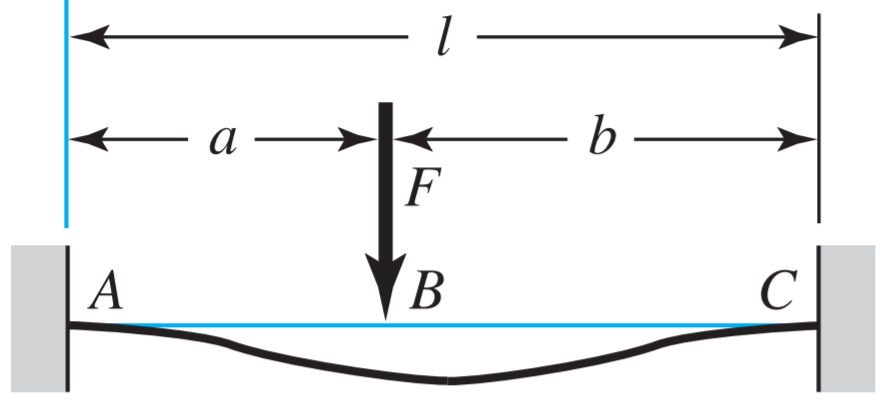
\includegraphics[width=0.7\linewidth]{../img/docs_beambend_btwn}
	\end{figure}
	
	With a force $ F $ applied perpendicularly at distance $ a $ from the left side of the beam and $ b $ from the right side, the deflection $ y $ at distance $ x $ from the left side is:
	
	\begin{gather}
	\begin{aligned}
		y\left( x \leq a \right) &= F \cdot \frac{b^2 x^2}{6 EI \cdot l^3} \left[ 3a l - x \left( 3a+b \right) \right] \\
		y\left( x \geq a \right) &= F \cdot \frac{a^2 \left( l - x \right)^2}{6 EI \cdot l^3} \left[ 3b l - \left( l - x \right) \left( 3b+a \right) \right]
	\end{aligned}
	\end{gather}
	\\
	Substitute $ b = l - a $, where $ a \leq \frac{l}{2} \leq b $:
	
	\begin{gather}
	\begin{aligned}
		y\left( x \leq a \right) &= F \cdot \frac{x^2 \left( l - a \right)^2}{6 EI \cdot l^3} \left[ 3a l - x \left( l + 2a \right) \right] \\
		y\left( x \geq a \right) &= F \cdot \frac{a^2 \left( l - x \right)^2}{6 EI \cdot l^3} \left[ 3x l - a \left( l + 2x \right) \right]
	\end{aligned}
	\end{gather}
	\\
	Taking the derivative of each and setting equal to zero, we find the local maxima of deflection:
	
	\begin{equation}
		x_{x \leq a} = 0,\ \frac{2al}{2a+l}\ ; \qquad\qquad
		x_{x \geq a} = \frac{l^2}{3l-2a},\ l
	\end{equation}
	\\
	At $ x = 0 $ and $ x = l $ the deflection is fixed at zero, so they cannot be the points of maxima. We must test the other solutions to make sure that they fulfil their domain requirements:
	
	\begin{gather}
	\begin{aligned}
		\frac{2al}{2a+l} \leq a &\implies a \geq \frac{l}{2}\ , \\
		\frac{l^2}{3l-2a} \geq a &\implies a \leq \frac{l}{2}\ \cup\ l \leq a \leq \frac{3}{2} l
	\end{aligned}
	\end{gather}
	\\
	The domain $ a \geq \frac{l}{2} $ for the first solution contradicts our definition of $ a \leq \frac{l}{2} \leq b $, therefore that solution is not valid. The second solution does not conflict, therefore it is valid and the maximum deflection occurs at $ x = \frac{l^2}{3l-2a} $. Plugging this into the corresponding deflection equation gives the maximum deflection for a beam supported on both sides:
	
	\begin{equation}
		y_{max} = \frac{2F a^2 \left( l - a \right)^3}{3 EI \left( 2a-3l \right)^2}
	\end{equation}
	
	\newpage
	We will now define a force on a beam supported only on one side. 
	
	\begin{figure}[H]
		\centering
		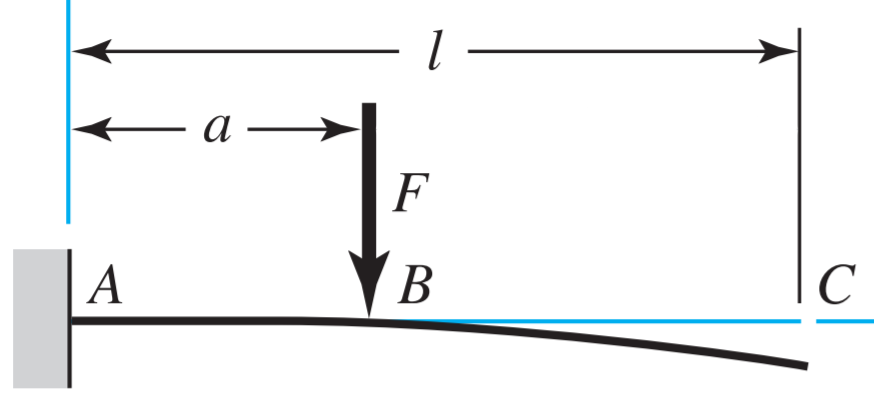
\includegraphics[width=0.7\linewidth]{../img/docs_beambend_cantilever}
	\end{figure}

	The beam is of length $ l $, fixed on the left side, with a force $ F $ applied perpendicularly at a distance of $ a $ away from the fixture. It is clear that the maximum deflection will occur at the right end of the beam. The magnitude of this deflection is represented by:
	
	\begin{equation}
		y_{max} = \frac{F a^2}{6 EI} \left( 3l - a \right)
	\end{equation}\\\\
	
	
	Again we will define a beam of length $ l $ supported only on one side, but this time we apply a twisting torque $ T $ at the opposite end.
	
	\begin{figure}[H]
		\centering
		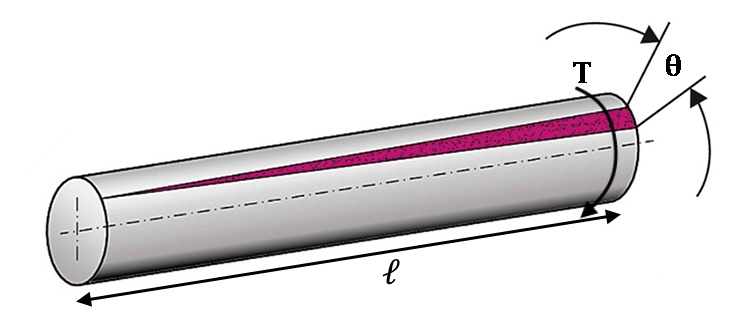
\includegraphics[width=0.7\linewidth]{../img/beambend_twist}
	\end{figure}

	This beam will deflect angularly along its axis. It is clear that the maximum angular deflection occurs at the end where the force is being applied. The magnitude of this deflection is:
	
	\begin{equation}
		\theta_{max} = \frac{T l}{GJ}
	\end{equation}\\
	
	
	
	
\end{document}